% Engineering Methods
%#cvicenie - opytat sa na cviceni
%ULOHA - treba spravit

\documentclass[11pt ,english,a4paper]{article}

\usepackage[english]{babel}
\usepackage[IL2]{fontenc}
\usepackage[utf8]{inputenc}
\usepackage{graphicx}
\usepackage{url}
\usepackage{hyperref}
\usepackage{times}
\usepackage{setspace}
\usepackage{float}

\setstretch{1.5}
\pagestyle{headings}

\title{Efficiency comparative analysis of techniques in misinformation detection in healthcare data\thanks{Semestral project in subject Engineering Methods, ac. year 2023/24, guidance: MSc. Mirwais Ahmadzai}}

\author{Alžbeta Žiarovská\\[2pt]
	{\small Slovak University of Technology in Bratislava}\\
	{\small Faculty of Informatics and Information Technologies}\\
	{\small \texttt{xziarovska@stuba.sk}}
	}

\date{\small 26. september 2023}



\begin{document}

\maketitle
\newpage

\begin{abstract}
\ldots
\end{abstract}
\newpage

\section{Introduction}\label{intro}

In this article I discuss the current situation regarding spread of misinformation in the medical field. This topic is very important in the aftermath of the global COVID-19 pandemic. More specifically I am making an analysis and comparison of different misinformation detection methods and their efficiency. During the pandemic we have seen a great rise of misinformation on the Internet, which provide danger to our society or even lives \cite{war18dr}. The main problem in my perception is, that the easy access to all the information on the Internet, which does not necessarily has to be true, can increase fear and anxiety and ultimately lead to the delay of diagnosis and receiving the effective healthcare in the case the information are not perceived correctly \cite{wa19sys}. 

I am focusing on comparing fact-checking and machine learning models as s way to find the medical misinformation. The fact-checking can be done manually or automatically which is introduced more deeply in Section \ref{tech:fact} \cite{bar21health}. The other side I am taking a closer look at are machine learning techniques including Naïve Bayes and Support Vector Machine \cite{bar21health}. I introduce these techniques and compare their efficiency in order to establish which one is the most suitable for healthcare misinformation detection.

In the Section \ref{mih} the term misinformation is described, how it differs from disinformation \cite{gu20misinfo}. Also a brief summary of historical development of misinformation spread is given \cite{pos18short}. It is also important to mention affect that medical fake news might have on our lives, which I address as well \cite{who22infodemics}. The last but not least, in Section \ref{tech}, I am taking a closer look at some of the methods used for misinformation recognition. I going to introduce them in a way, that would be easily understandable for all readers and state some of their outputs, so I can compare their effectiveness and possible impact for the future in Conclusion. \ref{conclusion}

\section{Misinformation in healthcare}\label{mih}

\paragraph{Difference between misinformation and disinformation}
The terms \emph{misinformation} and \emph{disinformation} are much the same, however, a small, but crucial difference can be distinguished. The difference between the two is a intention with which the false information is made accessible to the public and spread. Whilst the misinformation is usually created without direct intention of misleading and spreading false, meaning the person who put the information into the world might not actually know it is not true. On the other hand, disinformation is essentially created to spread false information. An example of such activity can be political propaganda \cite{gu20misinfo} \cite{cook15misinfo}. Even though the terms are not meaning the same, for the purpose of this article they are used as synonyms, because the author's knowledge, whether the information is factual, is negligible in the scope of its false recognition.

\paragraph{Historical development of concept of misinformation}%Lecture topic reaction
As the historical events have shown, the yearn for spreading not true information, either for amusement or with a goal of hurting someone, is old as a humanity itself \cite{bur17history}.

In the 16th century the writers have started to create completely false stories and plays in order to offer entertainment, but the drive was not only positive. During the French Revolution a rumor (in France called \emph{canard}) was used to discredit the queen Marie Antoinette, which doubtlessly did not help her in the later events of the French Revolution. \cite{bur17history} 

When the mass media took their place, the misleading was often used in order to change the opinion of the public during the times of war. For example during the World War II the Nazi propaganda was reaching the peaks of political propaganda ever. \cite{pos18short}

The rise of the \emph{hoax} in the era of the Internet is enormous and numerous fake websites were created.\cite{bur17history} Nowadays the information revolution by the Internet has brought many ways of spreading false information, but the way of their detection is not yet perfectly defined and therefore there is need for effective adaptive mechanisms.

\paragraph{Health care misinformation}%ULOHA
\cite{wa19sys}\cite{cook15misinfo} \cite{chap22unmask}
%Moreover,Internet content is fast becoming a replacement for expert advice,with a majority of Americans looking online for health information. However,numerous analyses of online content have found that a significant proportion of websites provide inaccurate medical information. \cite{cook15misinfo}
%and tobacco manufacturers have promoted misinformation about the public health impacts of smoking. \cite{cook15misinfo}

\paragraph{Societal context}%Lecture topic reaction
\cite{who22infodemics} page 8 \cite{wa19sys}


\section{Misinformation recognition techniques} \label{tech}

\subsection{Fact-checking technique} \label{tech:fact}
The process of fact-checking is used to distinguish, whether the specific claim is based on facts. This technique is usually used in a field of journalism \cite{alh18fact}.
There are two basic types of fact-checking to be differentiated:\cite{vla14fact} 
\begin{itemize}
\item Manual fact-checking
\item Automatic fact-checking
\end{itemize}
In subsection \ref{tech:fact:man} and \ref{tech:fact:auto} both of these will be introduced briefly.

\subsubsection{Manual fact-checking}\label{tech:fact:man}
Manual fact-checking is important process when we find some potentially false information on the Internet. However, it can be rather time consuming and usually ineffective way of finding factual information when the source is quite complex and contains a lot of detailed information \cite{gu22fact}. I offer a list of some of the basic points that can hold to in order to make the manual fact-checking as effective and quick as possible:
\begin{enumerate}
\item{\emph{Context}} - It is crucial to distinguish, whether the information is meant to be served as a fact to provide information or even to convince, or whether it is supposed to be taken as an exaggeration or sarcasm \cite{alh18fact}.
\item {\emph{Sentimental value}} - The goal of misinformation is often to scare people and spread panic. The difference between ratio of positive and negative in true and false claims is notable. Whilst in true claims the ratio is 71\% of positive words to 29\% of negative words, in misinformation sources this ratio is shifted the other way around with only 38\% of positive words and 62\% of negative words \cite{bar21health}.
\item {\emph{Sources}} - Perhaps the most important step might be to check the original sources of the claim \cite{gra17fact}. Anybody can share anything on the internet, so it is important to check, where does the information originally come from. We might need to look for the trustworthiness of the website or references, where did the author get the information from.
\end{enumerate}
In the figure \ref{f:man_fact} I created a mind map to illustrate the steps in process of manual fact-checking I enlisted in this section.

\begin{figure}[H]
\centering
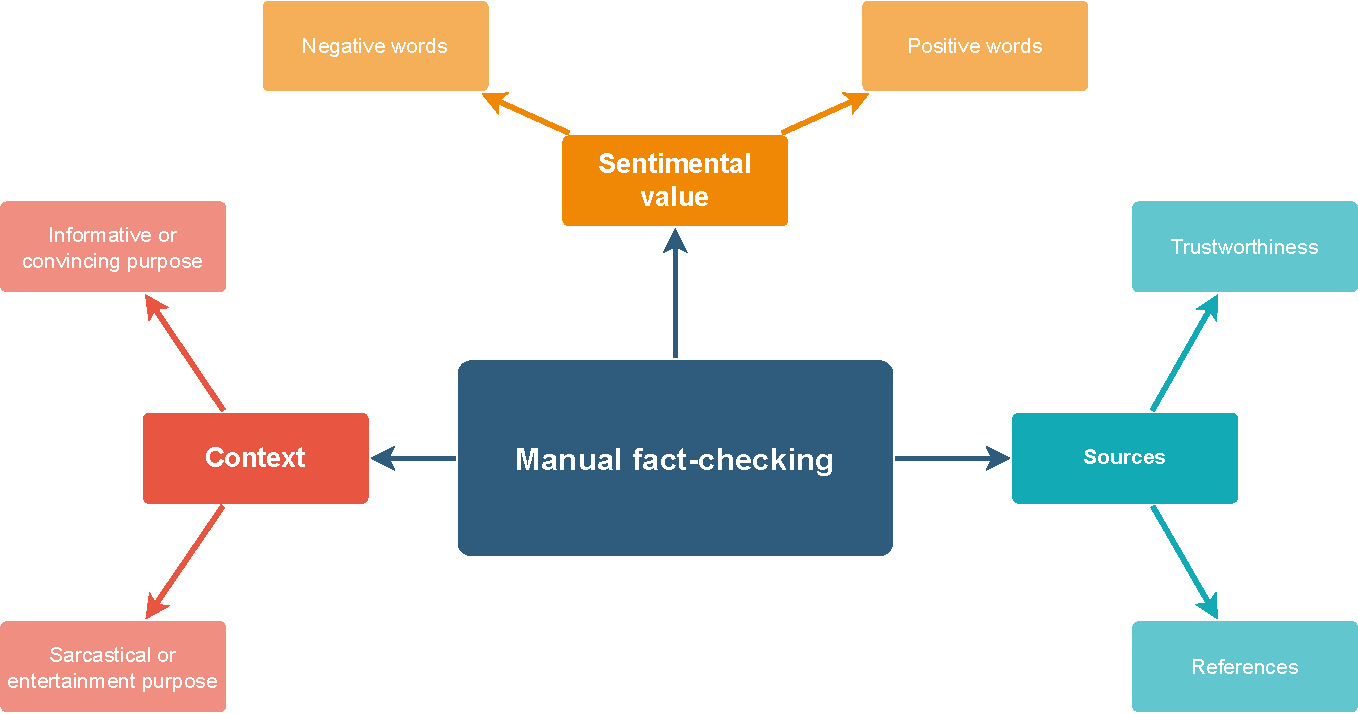
\includegraphics[scale=0.5]{manual_factchecking.pdf}
\caption{Mind map of Manual Fact-checking steps.}
\label{f:man_fact}
\end{figure}

\paragraph{Technology and people}%Lecture topic reaction
%backfire and boomerang page 5\cite{cook15misinfo}
%How can we benefit from manual fact-checking in out everyday lives

\subsubsection{Automatic fact-checking}\label{tech:fact:auto}
%websites FACTCHECK.org,POLITIFACT.comandFULLFACT.org \cite{alh18fact}
\cite{gu22fact}

\subsection{Machine learning techniques} \label{tech:mach}

%\paragraph{Definition}

%\paragraph{Text processing}

\subsubsection{Naïve Bayes}\label{nb}
The Naïve Bayes method is a linear probabilistic machine learning technique based on Bayes theorem. This method uses probability of the events without taking their relation into the consideration \cite{sha20mach}. This approach might not look to be the best, as the words have their order and are related one to other in articles. However, the opposite is true, as the linear models are capable of achieving high efficiency despite their simplicity \cite{pod19mach}. The accuracy of Naïve Bayes (as well as other machine learning methods) is also depended from which type of measuring the importance of the words in the documents is used. For the Naïve Bayes the result vary from 84,056\% \cite{sha20mach} to 98,71\% \cite{bar21health}. The closer analysis of these differences and their comparison is given in Section \ref{conclusion}.

Formula for Naïve Bayes calculation: \cite{sha20mach}

\begin{equation}
P(A|B) = \frac{P(B|A)P(A)}{P(B)}
\end{equation}

P(A\textbar B) is the probability of event A happening supposing, that event B has occurred.

\subsubsection{Support Vector Machine}\label{svm}
Support vector machine might be classified as a binary technique, as its methodology is to divide the data it was given into two categories \cite{pod19mach} (in the case of misinformation detection into true and false information). The division is made by creating a hyperplane (a object in the vector space with one dimension less, that the vector space itself \cite{sha20mach})
As it was mentioned in the section \ref{nb} about Naïve Bayes, the result can vary according to the technique used for analysis of the given data and for the Support Vector Machine numbers are on a scale from 83\% \cite{chap22unmask} to 95,05\% \cite{sha20mach}.

\paragraph{Ethics and sustainability}%Lecture topic reaction

\section{Conclusion}\label{conclusion}
%\cite{chap22unmask}
%\cite{bar21health} \cite{sha20mach} \cite{pod19mach}
%ULOHA - create a diagram to compare the accuracy of the models according to different sources (or make their average from the different sources and only put one info in the diagram, do not forget to put the equation of evaluating the average with reference to every number)

Je nejaké riešenie a aké?
Je vaše riešenie podobné iným (hoci aj z inej oblasti a len v z určitého hľadiska)?
O čom je článok, k čomu ste ním prispeli a čo zostáva otvorené?

%\acknowledgement{Ak niekomu chcete poďakovať\ldots}

\newpage
\bibliography{127323_bibliography}
\bibliographystyle{alpha} %alpha, abbrv
\end{document}
